% packages: none beyond core TikZ (explicit coordinates, core -latex arrow tips; renders on i.upmath.me as-is)
% Source of record for docs/figures/bnjettag-architecture.svg (rendered via the upmath MCP, 2026-08-23).
% Topology read from bnjettag/code/hgq2/bnhgq2/qat.py build_qat_model (input_proj, pos_enc, 2 encoder
% blocks, gap pool, head_fc1/2) and configs/r14-l1x3-n8-w1a8.json (d_model 32, 4 heads, ffn 64, norm none).
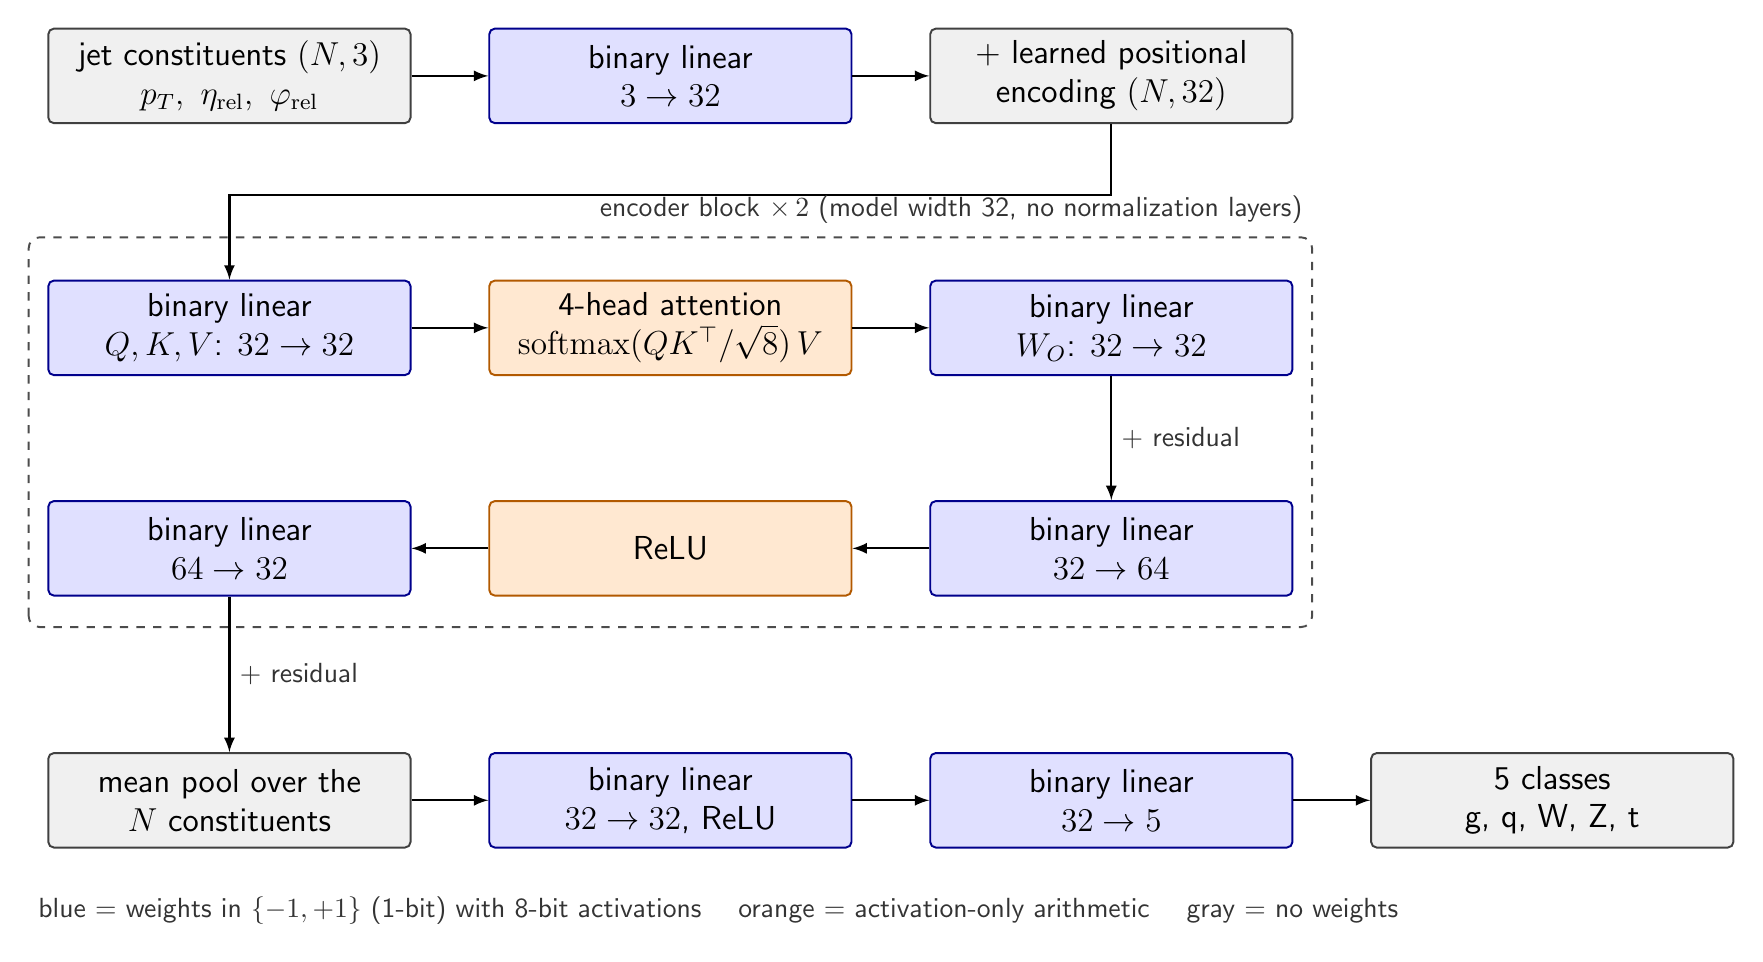
\begin{tikzpicture}[x=1cm,y=1cm,
  font=\sffamily\large,
  box/.style={draw, rounded corners=2pt, minimum height=12mm, minimum width=46mm, align=center, line width=0.7pt},
  bin/.style={box, fill=blue!12, draw=blue!55!black},
  act/.style={box, fill=orange!18, draw=orange!70!black},
  plain/.style={box, fill=gray!12, draw=gray!50!black},
  arr/.style={-latex, line width=0.8pt},
  lab/.style={font=\sffamily\normalsize, text=gray!40!black}
]
\node[plain] (in)   at (0,0)    {jet constituents $(N,3)$\\$p_T,\ \eta_{\mathrm{rel}},\ \varphi_{\mathrm{rel}}$};
\node[bin]   (proj) at (5.6,0)  {binary linear\\$3 \to 32$};
\node[plain] (pos)  at (11.2,0) {$+$ learned positional\\encoding $(N,32)$};
\node[bin]   (qkv)  at (0,-3.2)   {binary linear\\$Q,K,V$: $32\to32$};
\node[act]   (attn) at (5.6,-3.2) {4-head attention\\$\mathrm{softmax}(QK^{\top}/\sqrt{8})\,V$};
\node[bin]   (wo)   at (11.2,-3.2){binary linear\\$W_O$: $32\to32$};
\node[bin]   (fc1)  at (11.2,-6.0){binary linear\\$32\to64$};
\node[act]   (relu) at (5.6,-6.0) {ReLU};
\node[bin]   (fc2)  at (0,-6.0)   {binary linear\\$64\to32$};
\node[plain] (pool) at (0,-9.2)   {mean pool over the\\$N$ constituents};
\node[bin]   (h1)   at (5.6,-9.2) {binary linear\\$32\to32$, ReLU};
\node[bin]   (h2)   at (11.2,-9.2){binary linear\\$32\to5$};
\node[plain] (out)  at (16.8,-9.2){5 classes\\g, q, W, Z, t};
\draw[arr] (in) -- (proj);
\draw[arr] (proj) -- (pos);
\draw[arr] (pos.south) -- ++(0,-0.9) -| (qkv.north);
\draw[arr] (qkv) -- (attn);
\draw[arr] (attn) -- (wo);
\draw[arr] (wo) -- node[lab, right] {$+$ residual} (fc1);
\draw[arr] (fc1) -- (relu);
\draw[arr] (relu) -- (fc2);
\draw[arr] (fc2) -- node[lab, right] {$+$ residual} (pool);
\draw[arr] (pool) -- (h1);
\draw[arr] (h1) -- (h2);
\draw[arr] (h2) -- (out);
\draw[draw=gray!60!black, dashed, rounded corners=4pt, line width=0.7pt] (-2.55,-7.0) rectangle (13.75,-2.05);
\node[lab, anchor=south east] at (13.75,-2.0) {encoder block $\times\,2$ (model width 32, no normalization layers)};
\node[lab, anchor=north west] at (-2.55,-10.3) {blue = weights in $\{-1,+1\}$ (1-bit) with 8-bit activations \quad orange = activation-only arithmetic \quad gray = no weights};
\end{tikzpicture}
